% !TEX program = xelatex
% AY2014 材料力学 解答例（同志社 生命医科学 医工学コース 院試）
% 問題・図は 01_exams/2014/tex を土台に、参考/ の粒度で解答を付した。
\documentclass[11pt,a4paper]{article}
\usepackage{../../00_common/preamble}
\usetikzlibrary{positioning,arrows.meta,calc,patterns,decorations.pathmorphing}

\title{材料力学 AY2014 解答例}
\author{}
\date{}

\begin{document}
\maketitle

\noindent\textbf{符号規約}：はりでは反力・たわみは上向きを正，集中荷重 $P$ は下向き．
せん断力 $Q$ は断面左側に働く上向き外力の和，曲げモーメント $M$ は下に凸（さがり）を正とし，
たわみの基礎式は $EI_z\,\dfrac{d^2v}{dx^2}=M(x)$ を用いる．
軸力・軸応力は引張りを正，せん断応力・トルクは右ねじの向きを正とする．

%====================================================================
\section*{〔I〕}

A, C 点で支持されたはり（$A\,(x=0)$,\ $B\,(x=L)$,\ $C\,(x=2L)$,\ $D\,(x=3L)$，各区間 $L$）の
B 点に剛体アームが固定されている．剛体アームは B から高さ $a$ 上がり長さ $b$ 右へ伸び，
先端 E 点に下向きの集中荷重 $P$ が負荷される．はりの縦弾性係数を $E$，断面二次モーメントを $I_z$ とする．

\begin{center}
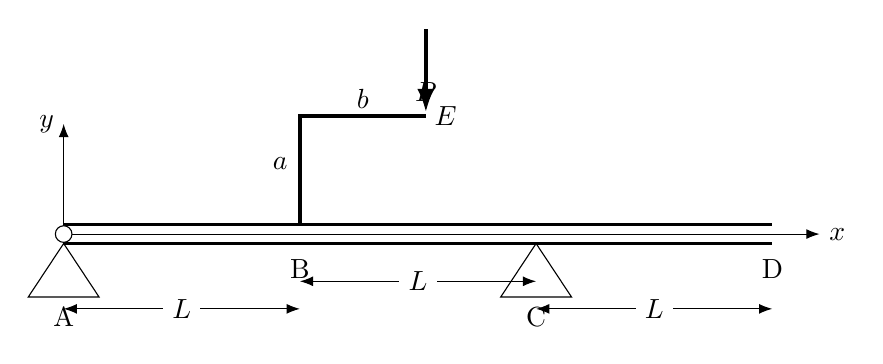
\begin{tikzpicture}[>=Latex]
  \draw[line width=1.2pt] (0,0.12) -- (9,0.12);
  \draw[line width=1.2pt] (0,-0.12) -- (9,-0.12);
  \draw[->] (0,0) -- (0,1.4) node[left]{$y$};
  \draw[->] (0,0) -- (9.6,0) node[right]{$x$};
  \draw[fill=white] (0,0) circle (3pt);
  \draw (0,-0.12) -- (-0.45,-0.8) -- (0.45,-0.8) -- cycle;
  \draw (6,-0.12) -- (5.55,-0.8) -- (6.45,-0.8) -- cycle;
  \draw[line width=1.6pt] (3,0.12) -- (3,1.5) -- (4.6,1.5);
  \node at (2.75,0.9) {$a$};
  \node at (3.8,1.72) {$b$};
  \node at (4.85,1.5) {$E$};
  \draw[->,very thick] (4.6,2.6) -- (4.6,1.55) node[above]{$P$};
  \node at (0,-1.05) {A};
  \node at (3,-0.45) {B};
  \node at (6,-1.05) {C};
  \node at (9,-0.45) {D};
  \draw[<->] (0,-0.95) -- (3,-0.95) node[midway,fill=white]{$L$};
  \draw[<->] (3,-0.6) -- (6,-0.6) node[midway,fill=white]{$L$};
  \draw[<->] (6,-0.95) -- (9,-0.95) node[midway,fill=white]{$L$};
\end{tikzpicture}

\vspace{2mm}
\begin{tikzpicture}[>=Latex,scale=0.9]
  \draw[fill=gray!15] (-0.5,-0.8) rectangle (0.5,0.8);
  \draw[->] (0,-0.8) -- (0,1.2) node[left]{$y$};
  \draw[->] (0,0) -- (-1.4,0) node[above]{$z$};
  \draw[<->] (-0.5,-1.05) -- (0.5,-1.05) node[midway,fill=white]{$w$};
  \draw[<->] (0.7,-0.8) -- (0.7,0.8) node[midway,fill=white]{$h$};
  \node at (0,-1.5) {断面};
\end{tikzpicture}

図1
\end{center}

\begin{enumerate}[label=(\arabic*)]
  \item 支持点 A, C における支持力を求めよ.
  \item はり AD 間のせん断力 $Q(x)$ と曲げモーメント $M(x)$ を求め，SFD と BMD を示せ.
  \item 幅 $w$，高さ $h$ の長方形断面とした場合，最大曲げ応力およびその発生位置の座標を求めよ.
  \item B 点および D 点におけるたわみを求めよ.
\end{enumerate}

\subsection*{解答}

\noindent\textbf{(1)}\quad 剛体アーム先端 E に作用する下向き荷重 $P$ を，固定点 B に等価に移すと，
\emph{下向きの力 $P$} と，水平距離 $b$ だけ離れていることによる\emph{偶力（モーメント）$M_0=Pb$}（時計回り）になる．
高さ $a$ は鉛直力に対して腕をもたないので寄与しない．

支点 A, C の上向き反力を $R_A,\ R_C$ とおく．鉛直方向のつり合いと，点 A まわりのモーメントのつり合い
（反時計回りを正，適用偶力は $-Pb$）より
\[
  R_A + R_C - P = 0, \qquad 2L\,R_C - L\,P - P\,b = 0 .
\]
第2式より $R_C=\dfrac{P(L+b)}{2L}$，これを第1式へ代入して
\[
  \ans{\,R_A=\frac{P(L-b)}{2L}\ (\text{上向き}),\qquad R_C=\frac{P(L+b)}{2L}\ (\text{上向き})\,}
\]
検算：点 C まわりのモーメント $-2L\,R_A+L\,P-Pb=-(L-b)P+LP-Pb=0$ ✓．

\medskip
\noindent\textbf{(2)}\quad 断面左側のつり合いを区間ごとにとる．B 点では下向き力 $P$ と偶力 $M_0=Pb$ が加わる．

\noindent(I)\ $0\le x<L$（区間 AB）：
\[
  Q(x)=R_A=\frac{P(L-b)}{2L},\qquad M(x)=R_A x=\frac{P(L-b)}{2L}\,x .
\]
\noindent(II)\ $L< x<2L$（区間 BC）：B 点で力 $P$（下向き）と偶力 $Pb$ が加わるので
\[
  Q(x)=R_A-P=-\frac{P(L+b)}{2L},\qquad
  M(x)=R_A x-P(x-L)+Pb=\frac{P(L+b)(2L-x)}{2L}.
\]
\noindent(III)\ $2L< x\le 3L$（区間 CD）：
\[
  Q(x)=R_A-P+R_C=0,\qquad M(x)=0 .
\]
（CD では荷重がなく自由端 D で $M=0$ ゆえ全区間 $M\equiv0$．）端点・接続点の値は
$M(0)=0$，$M(L^-)=\dfrac{P(L-b)}{2}$，$M(L^+)=\dfrac{P(L+b)}{2}$（B 点で偶力 $Pb$ の段差），$M(2L)=0$．
\[
  \ans{\,Q(x)=\begin{cases}\dfrac{P(L-b)}{2L} & (0\le x<L)\\[2mm]
   -\dfrac{P(L+b)}{2L} & (L<x<2L)\\[2mm] 0 & (2L<x\le 3L)\end{cases}
  \quad
  M(x)=\begin{cases}\dfrac{P(L-b)}{2L}\,x & (0\le x<L)\\[2mm]
   \dfrac{P(L+b)(2L-x)}{2L} & (L\le x\le 2L)\\[2mm] 0 & (2L\le x\le 3L)\end{cases}\,}
\]

\begin{center}
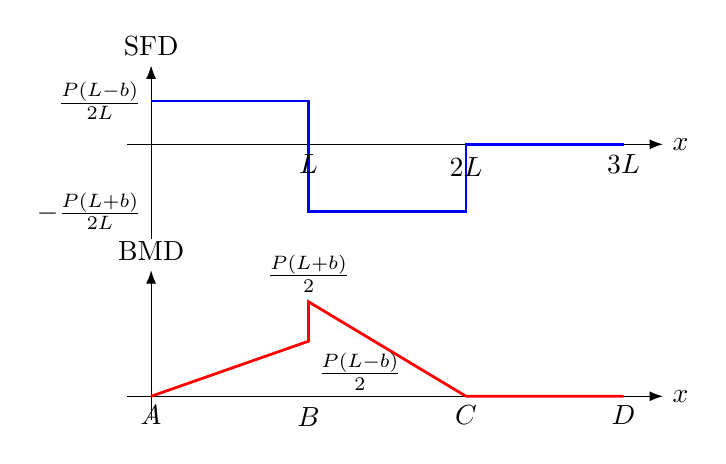
\begin{tikzpicture}[>=Latex,scale=1.0]
  \def\L{2.0}
  \begin{scope}
    \draw[->] (-0.3,0) -- (3*\L+0.5,0) node[right]{$x$};
    \draw[->] (0,-1.2) -- (0,1.0) node[above]{SFD};
    \draw[line width=1pt,blue] (0,0.55) -- (\L,0.55) -- (\L,-0.85) -- (2*\L,-0.85) -- (2*\L,0) -- (3*\L,0);
    \node[left] at (0,0.55) {$\frac{P(L-b)}{2L}$};
    \node[left] at (0,-0.85) {$-\frac{P(L+b)}{2L}$};
    \node[below] at (\L,0) {$L$}; \node[below] at (2*\L,-0.05) {$2L$}; \node[below] at (3*\L,0) {$3L$};
  \end{scope}
  \begin{scope}[yshift=-3.2cm]
    \draw[->] (-0.3,0) -- (3*\L+0.5,0) node[right]{$x$};
    \draw[->] (0,-0.3) -- (0,1.6) node[above]{BMD};
    \draw[line width=1pt,red] (0,0) -- (\L,0.7) -- (\L,1.2) -- (2*\L,0) -- (3*\L,0);
    \node[below right] at (\L,0.68) {$\frac{P(L-b)}{2}$};
    \node[above] at (\L,1.2) {$\frac{P(L+b)}{2}$};
    \node[below] at (0,0) {$A$}; \node[below] at (\L,-0.02) {$B$};
    \node[below] at (2*\L,0) {$C$}; \node[below] at (3*\L,0) {$D$};
  \end{scope}
\end{tikzpicture}
\end{center}

\medskip
\noindent\textbf{(3)}\quad 曲げモーメントの絶対値が最大となるのは B 点直右（$x=L$）で
\[
  |M|_{\max}=M(L^+)=\frac{P(L+b)}{2}.
\]
長方形断面の断面二次モーメントは $I_z=\dfrac{wh^3}{12}$，断面係数は $Z=\dfrac{I_z}{h/2}=\dfrac{wh^2}{6}$．したがって
\[
  \sigma_{\max}=\frac{|M|_{\max}}{Z}=\frac{P(L+b)/2}{wh^2/6}
  \quad\Longrightarrow\quad
  \ans{\,\sigma_{\max}=\frac{3P(L+b)}{w\,h^2}\,}
\]
発生位置は
\[
  \ans{\,x=L\ \text{の断面}（\text{B 点直右}），\ \text{上下縁}\ y=\pm\dfrac{h}{2}\,}
\]
（さがり $M>0$ なので $y=-h/2$ の下縁が最大引張り，$y=+h/2$ の上縁が最大圧縮．）
検算：$Z=\dfrac{wh^3/12}{h/2}=\dfrac{wh^2}{6}$ ✓．

\medskip
\noindent\textbf{(4)}\quad 基礎式 $EI_z v''=M(x)$ を各区間で2回積分する（$\times EI_z$ で表す）．
\[
  EI_z v_1=\frac{P(L-b)}{12L}x^3+C_1x+C_2\quad(0\le x\le L),
\]
\[
  EI_z v_2=\frac{P(L+b)}{2L}\!\left(Lx^2-\frac{x^3}{6}\right)+C_3x+C_4\quad(L\le x\le 2L),
\]
\[
  EI_z v_3=C_5x+C_6\quad(2L\le x\le 3L).
\]
境界条件 $v_1(0)=0$，$v_2(2L)=0$ と，B 点・C 点での連続条件
$v_1(L)=v_2(L),\ v_1'(L)=v_2'(L),\ v_2(2L)=v_3(2L),\ v_2'(2L)=v_3'(2L)$ で
$C_1\sim C_6$ を定めると，B 点（$x=L$）と D 点（$x=3L$）のたわみは
\[
  EI_z\,v_B=-\frac{PL^3}{6},\qquad
  EI_z\,v_D=\frac{PL^2(3L+b)}{12}.
\]
\[
  \ans{\,v_B=-\frac{PL^3}{6EI_z}\ (\text{下向き}),\qquad
   v_D=\frac{PL^2(3L+b)}{12EI_z}\ (\text{上向き})\,}
\]
検算：区間 CD では $Q=M=0$ なので CD は曲がらず，支点 C まわりに剛体的に回転する．
よって $v_D=v_C+\theta_C\cdot L=\theta_C L$ となり，傾き $\theta_C=v_3'$ から得た値と
$v_D=\dfrac{PL^2(3L+b)}{12EI_z}$ が一致する ✓．

%====================================================================
\clearpage
\section*{〔II〕}

長さ $L_1$，断面積 $A_1$，断面二次極モーメント $I_{p1}$，直径 $d_1$ の部分 AB と，
長さ $L_2$，断面積 $A_2$，$I_{p2}$，直径 $d_2$ の部分 BC からなる段付丸棒の両端 A, C を
剛体壁に固定する．同一材料で縦弾性係数 $E$，横弾性係数 $G$，熱膨張係数 $\alpha$．

\newcommand{\steppedshaft}{%
  \draw[line width=1pt] (0,-1.6) -- (0,1.6);
  \foreach \y in {-1.5,-1.2,...,1.55} {\draw (0,\y) -- (-0.28,\y+0.28);}
  \draw[line width=1pt] (8.5,-1.6) -- (8.5,1.6);
  \foreach \y in {-1.5,-1.2,...,1.55} {\draw (8.5,\y) -- (8.78,\y+0.28);}
  \draw[line width=1pt] (0,0.5) rectangle (4,-0.5);
  \draw[line width=1pt] (4,1.1) rectangle (8.5,-1.1);
  \draw[dash dot] (-0.6,0) -- (9.0,0);
  \draw[->] (0.6,0) -- (0.6,1.35) node[left]{$z$};
  \draw[->] (0.4,0) -- (1.5,0) node[above]{$x$};
  \draw (0.35,-0.35) circle (3.5pt); \draw (0.21,-0.49)--(0.49,-0.21); \draw (0.21,-0.21)--(0.49,-0.49);
  \node[below left] at (0.35,-0.5) {$y$};
  \node at (0.55,0.75) {A}; \node at (4.0,1.35) {B}; \node at (8.2,1.35) {C};
  \node at (2.0,-0.25) {$A_1\ \ I_{p1}$};
  \node at (6.2,-0.55) {$A_2\ \ I_{p2}$};
  \draw[<->] (0,-1.35) -- (4,-1.35) node[midway,fill=white]{$L_1$};
  \draw[<->] (4,-1.35) -- (8.5,-1.35) node[midway,fill=white]{$L_2$};
}

\begin{center}
\begin{tikzpicture}[>=Latex,scale=0.82]
  \steppedshaft
\end{tikzpicture}

図2\qquad
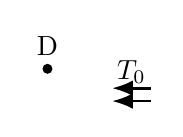
\begin{tikzpicture}[>=Latex,scale=0.82]
  \steppedshaft
  \fill (2,0.5) circle (2.2pt);
  \node[above] at (2,0.55) {D};
  \draw[->,line width=1pt] (3.6,0.2) -- (3.0,0.2);
  \draw[->,line width=1pt] (3.6,0.0) -- (3.0,0.0);
  \node at (3.3,0.45) {$T_0$};
\end{tikzpicture}

図3
\end{center}

\begin{enumerate}[label=(\arabic*)]
  \item 温度を $\Delta T$ 上昇させた時，部分 AB, BC に生じる熱応力 $\sigma_1,\ \sigma_2$ を求めよ.
  \item 図3のように断面 B にトルク $T_0$ が作用する時，支持トルク $T_A,\ T_C$，最大せん断応力
        $\tau_{AB},\ \tau_{BC}$，B 点のねじれ角 $\Psi_B$ を求めよ.
  \item $\Delta T$ 上昇かつ $T_0$ 作用時，点 D$\left(\frac{L_1}{2},0,\frac{d_1}{2}\right)$ における
        微小要素の応力とモールの応力円を求め，$\sigma_{\max},\ \tau_{\max}$ を求めよ.
\end{enumerate}

\subsection*{解答}

\noindent\textbf{(1)}\quad 両端が剛体壁に固定されているので，棒全体の軸方向変位は 0 である（静定不可）．
軸力 $N$（引張り正，全長で一定）とすると，自由熱膨張と弾性変形の和が 0：
\[
  \alpha\,\Delta T\,(L_1+L_2)+\frac{N L_1}{E A_1}+\frac{N L_2}{E A_2}=0 .
\]
これを解いて
\[
  N=-\frac{\alpha\,\Delta T\,(L_1+L_2)}{\dfrac{L_1}{EA_1}+\dfrac{L_2}{EA_2}}
   =-\frac{E\,\alpha\,\Delta T\,(L_1+L_2)}{\dfrac{L_1}{A_1}+\dfrac{L_2}{A_2}}\ (<0,\ \text{圧縮}).
\]
熱応力 $\sigma_1=N/A_1,\ \sigma_2=N/A_2$ は
\[
  \ans{\,\sigma_1=-\frac{E\,\alpha\,\Delta T\,(L_1+L_2)}{\,L_1+\dfrac{A_1}{A_2}L_2\,},\qquad
        \sigma_2=-\frac{E\,\alpha\,\Delta T\,(L_1+L_2)}{\,L_2+\dfrac{A_2}{A_1}L_1\,}\,}
\]
ともに負（圧縮）である．検算：軸力一定より $\sigma_1 A_1=\sigma_2 A_2=N$ が成り立つ ✓．

\medskip
\noindent\textbf{(2)}\quad A, C の支持トルクを $T_A,\ T_C$ とする．つり合いと適合条件は
\[
  T_A+T_C=T_0,\qquad
  \underbrace{\frac{T_A L_1}{G I_{p1}}}_{\text{B の A に対するねじれ}}
   =\underbrace{\frac{T_C L_2}{G I_{p2}}}_{\text{B の C に対するねじれ}} .
\]
これを解くと（$D\equiv L_1 I_{p2}+L_2 I_{p1}$ とおく）
\[
  \ans{\,T_A=\frac{T_0 L_2 I_{p1}}{L_1 I_{p2}+L_2 I_{p1}},\qquad
        T_C=\frac{T_0 L_1 I_{p2}}{L_1 I_{p2}+L_2 I_{p1}}\,}
\]
各部の内部トルクは AB が $T_A$，BC が $T_C$．最大せん断応力 $\tau=\dfrac{T\,(d/2)}{I_p}$ は
\[
  \ans{\,\tau_{AB}=\frac{T_0 L_2\,d_1}{2\,(L_1 I_{p2}+L_2 I_{p1})},\qquad
        \tau_{BC}=\frac{T_0 L_1\,d_2}{2\,(L_1 I_{p2}+L_2 I_{p1})}\,}
\]
B 点のねじれ角は
\[
  \Psi_B=\frac{T_A L_1}{G I_{p1}}=\frac{T_0 L_1 L_2}{G\,(L_1 I_{p2}+L_2 I_{p1})}
  \quad\Longrightarrow\quad
  \ans{\,\Psi_B=\frac{T_0 L_1 L_2}{G\,(L_1 I_{p2}+L_2 I_{p1})}\,}
\]
（支持トルク $T_A,\ T_C$ は $T_0$ と逆向きに，それぞれ A, C で壁から作用する．）
検算：$T_A+T_C=\dfrac{T_0(L_2 I_{p1}+L_1 I_{p2})}{L_1 I_{p2}+L_2 I_{p1}}=T_0$，
かつ $\dfrac{T_A L_1}{GI_{p1}}=\dfrac{T_C L_2}{GI_{p2}}=\Psi_B$ が成り立つ ✓．

\medskip
\noindent\textbf{(3)}\quad 点 D は部分 AB の表面（$x=L_1/2$，半径 $d_1/2$）にある．
この点の微小要素には，軸方向の熱応力 $\sigma_x=\sigma_1$（圧縮）と，
AB 内のトルク $T_A$ によるねじりせん断応力 $\tau_{xy}=\tau_{AB}$ が生じる（$\sigma_y=0$）．
\[
  \sigma_x=\sigma_1=-\frac{E\,\alpha\,\Delta T\,(L_1+L_2)}{L_1+\frac{A_1}{A_2}L_2},\qquad
  \tau_{xy}=\tau_{AB}=\frac{T_0 L_2\,d_1}{2(L_1 I_{p2}+L_2 I_{p1})}.
\]
平面応力のモール円は，中心 $C=\dfrac{\sigma_x}{2}$，半径 $R=\sqrt{\left(\dfrac{\sigma_x}{2}\right)^2+\tau_{xy}^2}$．
主応力・最大せん断応力は
\[
  \ans{\,\sigma_{\max}=\frac{\sigma_x}{2}+\sqrt{\left(\frac{\sigma_x}{2}\right)^2+\tau_{xy}^2},
   \qquad
   \tau_{\max}=\sqrt{\left(\frac{\sigma_x}{2}\right)^2+\tau_{xy}^2}\,}
\]
（最小主応力は $\sigma_{\min}=\dfrac{\sigma_x}{2}-R$．$\sigma_x<0$ なので円の中心は $\sigma$ 軸の負側にある．）

\begin{center}
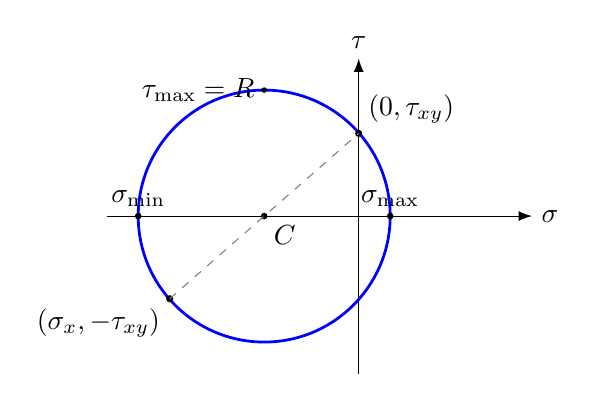
\begin{tikzpicture}[>=Latex,scale=1.0]
  % 軸
  \draw[->] (-3.2,0) -- (2.2,0) node[right]{$\sigma$};
  \draw[->] (0,-2.0) -- (0,2.0) node[above]{$\tau$};
  % 中心 (-1.2,0), 半径 1.6
  \def\cx{-1.2}\def\rr{1.6}
  \draw[blue,line width=1pt] (\cx,0) circle (\rr);
  \fill (\cx,0) circle (1.2pt); \node[below right] at (\cx,0) {$C$};
  % 状態点 (σx, -τ) と (0, τ)
  \fill (-2.4,-1.05) circle (1.3pt); \node[below left] at (-2.4,-1.05) {$(\sigma_x,-\tau_{xy})$};
  \fill (0,1.05) circle (1.3pt); \node[above right] at (0,1.05) {$(0,\tau_{xy})$};
  \draw[gray,dashed] (-2.4,-1.05) -- (0,1.05);
  % σmax, σmin, τmax
  \fill (\cx+\rr,0) circle (1.2pt); \node[above] at (\cx+\rr,0) {$\sigma_{\max}$};
  \fill (\cx-\rr,0) circle (1.2pt); \node[above] at (\cx-\rr,0) {$\sigma_{\min}$};
  \node[left] at (\cx,\rr) {$\tau_{\max}=R$};
  \fill (\cx,\rr) circle (1.0pt);
\end{tikzpicture}

モールの応力円（模式図）
\end{center}
検算：$\sigma_{\max}+\sigma_{\min}=\sigma_x$（不変量），$\sigma_{\max}-\sigma_{\min}=2R=2\tau_{\max}$ が
成り立つ ✓．

\end{document}
